\subsubsection{Load Transfer Configuration Study}

Accurate thrust measurement in a test stand structure can prove to be a greater challenge than it may seem due to the nature of structural load transfer. Any applied forces or loads will pass through any and all available structural paths, travelling from the point in which the loads are applied, towards the fixed part of the test stand. If the test stand built in a statically determinant configuration, thrust loads can be measured to a higher accuracy, depending entirely on the geometry of the engine interface.

However, true statically determinate systems are largely uncommon in real-world applications, so thrust structures tend to be built in a statically indeterminate configuration. In this case, the load transfer through a given structure depends on the geometry of the interface as well as the stiffness of the load paths in question. This trade study focuses on the nature of the test stand’s structural interface, and different potential configurations that will minimize the effects of load path stiffness that comes with a statically indeterminate test stand configuration.

\noindent\underline{Option 1: Static Structure/Floating Plate Configuration}

A static structure/floating plate configuration consists of two main sections, a “floating plate” in which the test article is attached to in order to reduce the amount of interface stiffness, and the static structure, which essentially consists of the rest of the test stand and is where the stand will be constrained to the ground/a tabletop. These two sections are connected with the load cell(s), in which most of the axial stiffness is transferred through, to ensure the thrust measurements are as accurate as possible. The floating plate may also be connected to the static structure with additional flexures, as long as the flexures are designed in a way to ensure minimum axial stiffness through the floating plate itself while still supporting the test article against any transverse loads (such as the weight of the test article itself).

\begin{figure}
    \centering
    \raisebox{-0.5\height}{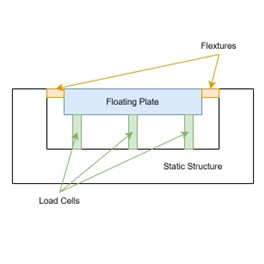
\includegraphics[width=0.4\linewidth]{static-structure-floating-plate-diagram.jpg}}
    \hspace{3em}
    \raisebox{-0.5\height}{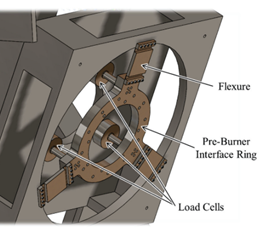
\includegraphics[width=0.4\linewidth]{static-structure-floating-plate-example.png}}
    \caption{\centering{A diagram of the static structure/floating plate configuration (left) and an example developed by Purdue's Zucrow Labs (right).}}
    \label{fig:static-floating-plate-example}
\end{figure}

\noindent\textit{Pros:}

The static structure/floating plate configuration is a very compact and straightforward design, stemming from the floating plate that transmits any thrust force directly to the load cells. This configuration reduces the number of moving parts in the system as a whole, which minimizes potential points of failure and makes the system easier to implement and maintain. This is particularly advantageous for facilities with limited space or those requiring a simple and straightforward solution.

One major strength of this configuration lies in its accuracy for axial force measurements while being able to minimize potential distortions caused by friction much easier. Compared to more complicated systems, this configuration reduces parasitic forces caused by structural deflections and alignment issues more efficiently as well. Because the test article is more closely anchored to the static structure, it is able to provide much more stability and ensure repeatable results over multiple tests.

With no sliding or other wear-prone components, this configuration would also be highly durable. This will ensure a much longer operational lifespan with minimal degradation or needed maintenance, which makes this configuration particularly suited for high-frequency testing environments. The lack of moving parts also makes the system less vulnerable to environmental factors, such as dust or debris, which could interfere with the operation of more complex configurations.

\noindent\textit{Cons:}

The first and foremost drawback of this configuration is how the floating plate will need to be specifically tailored to ensure it can integrate with each test article. While it is possible to keep integration methods the same between each test article, the floating plate design could limit the potential maximum size and thrust production that the test stand could handle. Retrofitting the test stand may require significant effort, making it less ideal for facilities conducting tests on a wide variety of test articles.

Another limitation lies in this configuration’s ability to handle dynamic or multi-axis forces. While a sliding rail configuration could be configured in a way to handle these extra forces, this design would only really be able to capture the axial force in a single direction without major modifications to the sensor system. In a project where budget is limited, compensating for the lack of dynamic force detection with multiple load cells may not be a great option.

There may also be a negative impact on this configuration caused by structural deformation and thermal effects. While the static structure provides a stable base for the test article, engines producing a particularly high thrust can induce minor deflections in the floating plate, potentially affecting the measurement accuracy. Addressing these issues often requires careful material selection and design, adding cost and complexity to what is otherwise a cost-effective and straightforward configuration.

\noindent\underline{Option 2: Sliding Rail Configuration}

A sliding rail configuration consists of a platform or carriage in which the test article is mounted on, and then this platform would slide along rails or bearings. The rails or bearings would be made out of low-friction materials (e.g. Teflon), to ensure accurate force transfer without any distortion caused by parasitic forces. The platform or carriage would then push into load cells attached to the rest of the test stand in order to measure the axial thrust generated by the test article. By putting the test article on rails or bearings, any forces produced would be constrained to the axial thrust direction, which allows the forces to be more accurately directed into the load cells.

\begin{figure}
    \centering
    \raisebox{-0.5\height}{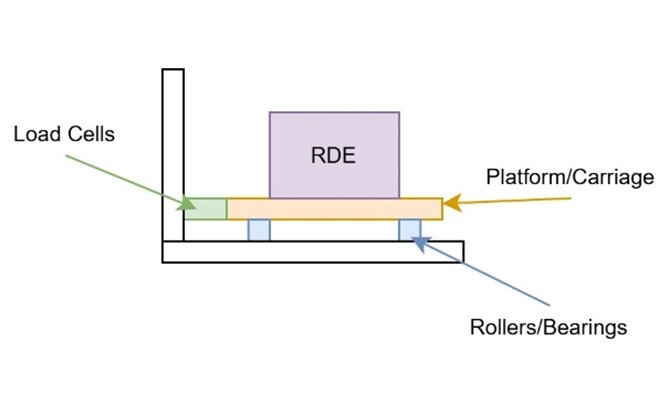
\includegraphics[width=0.4\linewidth]{sliding-rail-diagram.jpg}}
    \hspace{3em}
    \raisebox{-0.5\height}{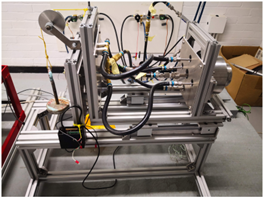
\includegraphics[width=0.4\linewidth]{sliding-rail-example.png}}
    \caption{\centering{A diagram of the sliding rail configuration (left) and an example developed by the University of Southampton (right).}}
    \label{fig:sliding-rail-example}
\end{figure}

\noindent\textit{Pros:}

The sliding rail configuration is one of the most ideal choices for isolating and accurately measuring axial forces generated by the test article. By constraining the test article’s motion to a single axis through rails or bearings, the system ensures that thrust is directed cleanly to the load cells, minimizing any interference from lateral forces. Using low-friction sliders or bearings also reduces the effect of parasitic forces such as friction. This allows for high-fidelity thrust measurements, where even minor distortions in force pathways could compromise the results.

This configuration also has the advantage of being modular and adaptable. The design can be easily adjusted to accommodate test articles of various sizes or thrust levels, which is particularly useful for a testing campaign with the goal of rapidly iterating over different designs, with each design able to be quickly integrated with the test stand numerous times. This dynamic testing environment of variable engine size/thrust can prove to be very useful for analyzing engine performance under realistic operating conditions.

The use of rails would also minimize structural distortion, as any thrust produced by the test article will be isolated to the rails and load cells, rather than being absorbed by a rigid frame. This will ensure consistent measurements, even for high-thrust engines, without the risk of inaccuracies from structural deformation. Additionally, the platform or sled in which the test article is integrated with will aid with thermal management by reducing heat transfer to the load cells and rest of the test stand structure.

\noindent\textit{Cons:}

One of the more major concerns that must be addressed with a sliding rail test stand configuration is the complexity of alignment. The rails and platform that the test article is on must be precisely aligned in order to ensure smooth motion and accurate force transmission into the load cells. Any improper alignment can introduce measurement errors, or worse, cause mechanical binding in the rail or bearing system. The demand for high precision increases initial installation time and the need for ongoing adjustments.

In addition, maintenance requirements could prove to increase the complexity required to implement the sliding rail solution. Any sliding components must be regularly inspected, cleaned, and lubricated in order to maintain their low-friction properties and ensure consistent performance. Over time, foreign object debris and wear and tear within the sliding components can lead to increased resistance, introducing additional parasitic forces that distort the thrust measurements.

While the nature of keeping the test article integrated to a separate platform will greatly reduce the amount of heat that transfers to the rest of the test stand, there could still be a non-negligible amount of heat that transfers to the rails. Any excessive heat that transfers to the sliding mechanism could potentially cause thermal expansion or warping, which would negatively affect the precise alignment and measurement accuracy. While this issue can be mitigated with proper material selection and thermal insulation techniques, it makes the sliding rail configuration less ideal for applications where simplicity and cost are major priorities.

% ----- CRITERIA & WEIGHTS -----
\begin{table}[H]
    \centering
    \singlespacing
    \small
    \caption{Load Transfer Configuration Trade Study - Evaluation Criteria}
    \label{tab:load_transfer_config_eval_criteria}

    \begin{subtable}[t]{\linewidth}
        \begin{tabularx}{\linewidth}{
            |>{\hsize=0.200\hsize}>{\centering\arraybackslash}X
            |>{\hsize=0.100\hsize}>{\centering\arraybackslash}X
            |>{\hsize=0.700\hsize}>{\centering\arraybackslash}X|
        }
            \hline
            \textbf{Decision Criteria} & \textbf{Weight} & \textbf{Reason} \\ \hline

            Complexity & 15\% & The design needs to be able to achieve its goals without unnecessary complexity in its assembly, serviceability, or maintenance, that can yield extra failure modes or unexpected behavior. \\ \hline
        
            Manufacturability & 15\% & The test stand should be able to be machined at the UCF machine shop without added difficulty. \\ \hline
        
            Risk & 20\% & While each option being considered has been tested in research previously, their specific adaptation to SABR can and will introduce unexpected risks, making the configuration choice paramount. \\ \hline
        
            Technical Performance & 50\% & The design’s ability to reliably handle and accurately measure the thrust produced by SABR are crucial for the success of the project. \\ \hline
        \end{tabularx}
        \smallskip
        \caption{Evaluation Criteria and Weights}
    \end{subtable}

\end{table}

\vspace{-2em}

% ----- COMPLEXITY SCALE -----
\begin{table}[H]
    \centering
    \singlespacing
    \small
    \ContinuedFloat

    \begin{subtable}[t]{\linewidth}
        \begin{tabularx}{\linewidth}{
            |>{\hsize=0.150\hsize}>{\centering\arraybackslash}X
            |>{\hsize=0.850\hsize}>{\centering\arraybackslash}X|
        }
            \hline
            \textbf{Score} & \textbf{Reason} \\ \hline
        
            4 & The design is simple in assembly, integration, use, and maintenance. \\ \hline
            
            3 & The design remains simple in assembly, integration and use, but maintenance requires some thought. \\ \hline
            
            2 & The design requires careful thought when integrating the engine or performing maintenance, but no critical issues arise from failure in these areas. \\ \hline
            
            1 & The design requires extreme care when assembling, integrating the engine, or performing maintenance, and poses a risk if these needs are not met. \\ \hline
        \end{tabularx}
        \smallskip
        \caption{Evaluation Scale - Complexity}
    \end{subtable}
\end{table}

\vspace{-2em}

% ----- MANUFACTURABILITY SCALE -----
\begin{table}[H]
    \centering
    \singlespacing
    \small
    \ContinuedFloat

    \begin{subtable}[t]{\linewidth}
        \begin{tabularx}{\linewidth}{
            |>{\hsize=0.150\hsize}>{\centering\arraybackslash}X
            |>{\hsize=0.850\hsize}>{\centering\arraybackslash}X|
        }
            \hline
            \textbf{Score} & \textbf{Reason} \\ \hline
        
            4 & The design remains functional with simple manufacturing methods and precise location of interacting components is not necessary. \\ \hline
            
            3 & The design remains functional with simple manufacturing methods and precise location and alignment is not necessary, but integration is critical to performance. \\ \hline
            
            2 & Manufacturing is complex but achievable within the means available; the design requires careful planning for integration and misalignment affects performance. \\ \hline
            
            1 & The design requires extreme care in integration and alignment of interacting components to maintain performance. Manufacturing is difficult and requires special tooling/machinery. \\ \hline
        \end{tabularx}
        \smallskip
        \caption{Evaluation Scale - Manufacturability}
    \end{subtable}
\end{table}

\vspace{-2em}

% ----- RISK SCALE -----
\begin{table}[H]
    \centering
    \singlespacing
    \small
    \ContinuedFloat

    \begin{subtable}[t]{\linewidth}
        \begin{tabularx}{\linewidth}{
            |>{\hsize=0.150\hsize}>{\centering\arraybackslash}X
            |>{\hsize=0.850\hsize}>{\centering\arraybackslash}X|
        }
            \hline
            \textbf{Score} & \textbf{Reason} \\ \hline
        
            4 & The design does not pose any risk to the structural stability of the test stand, and parasitic force distribution through the test stand is unlikely. \\ \hline
            
            3 & The design does not pose any risk to the structural stability of the test stand, but parasitic force distribution through the test stand is possible. \\ \hline
            
            2 & The design poses somewhat of a risk to the structural stability of the test stand, and parasitic force distribution is almost guaranteed. \\ \hline
            
            1 & The design poses an extreme risk to the structural stability of the test stand, and parasitic force distribution is almost guaranteed. \\ \hline
        \end{tabularx}
        \smallskip
        \caption{Evaluation Scale - Risk}
    \end{subtable}
\end{table}

\vspace{-2em}

% ----- TECHNICAL PERFORMANCE SCALE -----
\begin{table}[H]
    \centering
    \singlespacing
    \small
    \ContinuedFloat

    \begin{subtable}[t]{\linewidth}
        \begin{tabularx}{\linewidth}{
            |>{\hsize=0.150\hsize}>{\centering\arraybackslash}X
            |>{\hsize=0.850\hsize}>{\centering\arraybackslash}X|
        }
            \hline
            \textbf{Score} & \textbf{Reason} \\ \hline
        
            4 & The design exceeds the desired thrust measurement requirements for SABR performance. \\ \hline
            
            3 & The design meets the minimum thrust measurement requirements for SABR performance. \\ \hline
            
            2 & The design can meet the minimum thrust measurement requirements for SABR performance but requires a significant amount of post-processing on the load cell data. \\ \hline
            
            1 & The design is inefficient, ineffective, or otherwise fails to meet the desired thrust measurement requirements for SABR. \\ \hline
        \end{tabularx}
        \smallskip
        \caption{Evaluation Scale - Technical Performance}
    \end{subtable}
\end{table}

\vspace{-2em}

% ----- DECISION MATRIX (W/ COLORS) -----
% \begin{table}[H]
%     \centering
%     \singlespacing
%     \small
%     \begin{tabular}{|c|c|c|c|}

%         \hline
%         \multicolumn{2}{|c|}{\textbf{Criteria and Weights}}                         & \multicolumn{2}{|c|}{\textbf{Options and Scores}}                     \\ \hline

%         \textbf{Criteria}                                       & \textbf{Weights}  & \textbf{Static/Floating Plate}    & \textbf{Sliding Rail}             \\ \hline

%         \multicolumn{1}{|l|}{\textbf{Complexity}}               & 0.15              & \cellcolor{green!85!black} 4      & \cellcolor{green!15!yellow} 3     \\ \hline

%         \multicolumn{1}{|l|}{\textbf{Manufacturability}}        & 0.15              & \cellcolor{green!85!black} 4      & \cellcolor{green!15!yellow} 3     \\ \hline

%         \multicolumn{1}{|l|}{\textbf{Risk}}                     & 0.20              & \cellcolor{green!15!yellow} 3     & \cellcolor{green!85!black} 4      \\ \hline

%         \multicolumn{1}{|l|}{\textbf{Technical Performance}}    & 0.50              & \cellcolor{green!85!black} 4      & \cellcolor{green!85!black} 4      \\ \Xhline{2pt}

%         \multicolumn{1}{|l|}{\textbf{Weighted Scores}}          &                   & \cellcolor{green!85!black} 3.8    & \cellcolor{green!15!yellow} 3.7   \\ \hline

%     \end{tabular}
%     \caption{Load Transfer Configuration Study - Decision Matrix}
%     \label{tab:load_transfer_config_decision_matrix}
% \end{table}

% ----- DECISION MATRIX (W/O COLORS) -----
\begin{table}[H]
    \centering
    \singlespacing
    \small
    \begin{tabularx}{0.8\linewidth}{
        |>{\hsize=0.35\hsize}>{\centering\arraybackslash}X
        |>{\hsize=0.15\hsize}>{\centering\arraybackslash}X
        |>{\hsize=0.25\hsize}>{\centering\arraybackslash}X
        |>{\hsize=0.25\hsize}>{\centering\arraybackslash}X|
    }
        \hline
        \multicolumn{2}{|c|}{\textbf{Criteria and Weights}} & \multicolumn{2}{|c|}{\textbf{Options and Scores}} \\ \hline

        \textbf{Criteria} & \textbf{Weights} & \textbf{Hydraulic Calibration Structure} & \textbf{Mass-Pulley Calibration Structure} \\ \hline

        \multicolumn{1}{|l|}{\textbf{Complexity}} & 0.15 & 4 & 3 \\ \hline

        \multicolumn{1}{|l|}{\textbf{Manufacturability}} & 0.15 & 4 & 3 \\ \hline

        \multicolumn{1}{|l|}{\textbf{Risk}} & 0.20 & 3 & 4 \\ \hline

        \multicolumn{1}{|l|}{\textbf{Technical Performance}} & 0.50 & 4 & 4 \\ \Xhline{2pt}

        \multicolumn{1}{|l|}{\textbf{Weighted Scores}} & & 3.8 & 3.7 \\ \hline
        
    \end{tabularx}
    \caption{Load Transfer Configuration Study - Decision Matrix}
    \label{tab:load_transfer_config_decision_matrix}
\end{table}

\noindent\underline{Decision}

As shown by the decision matrix, the static structure/floating plate system is the optimal choice for the load transfer configuration. This system is much less complex from a design and integration standpoint, is much easier to manufacture and assemble, and is expected to yield the same results as the sliding rail configuration from a data measurement standpoint. Despite the slightly increased level of risk associated with this configuration, it is outweighed by its lack of complexity and cost. The decision to use a sliding rail configuration would yield similar results for thrust measurement, but the added complexity required to achieve that result is much less ideal.